%   File: Babyboot.tex
% Author: Adam Leeper (with modifications by Paul Mitiguy)
%------------------------------------------------------------------------------
%\\[0.45pc]
\providecommand{\isolatedBuild}[1]{#1}% Fallback definition to build normally.
\isolatedBuild{
  \documentclass[11pt,letterpaper]{book}
  %\documentclass[11pt,letterpaper]{book}

% aleeper: I think these are needed for Paul's macros?
\usepackage{epsfig}
\usepackage{epstopdf}

%\makeatletter
%\typeout{The import path is \import@path}
%\makeatother

\usepackage{import}

\subimport{./}{packagesMitiguy.sty}
\subimport{./}{macrosMitiguy.tex}
\subimport{./}{PageStylesMitiguy.tex}
\subimport{./}{macrosLeeper.tex}
   % Found via TEXINPUTS environment variable.
  \isolatedBuildHeader{Angular Acceleration}
                      {Angular Acceleration of a Babyboot Pendulum}
}
%%%
%%%
%%%
\begin{minipage}[t]{0.6\textwidth}
  \minipageTopAnchor
  A babyboot pendulum (as shown in class) is pictured at right,
  consisting of a rod \basis{A} and rectangular plate \basis{B}.
  Assume the support structure is a Newtonian reference frame \basis{N}.
  Sets of right-handed  orthogonal unit vectors are fixed in each frame as shown,
  and angles $\theta$ and $\phi$ are indicated on the figure.
  \\[0.45pc]
  To help clarify the figure:
  $\theta$ is the angle between \uvecz{n} and \uvecz{a} with $+\uvecx{a}$ sense,
  and $\phi$ is the angle between \uvecx{a} and \uvecx{b} with $+\uvecz{b}$ sense.
  %\\[0.5pc]
  %Clearly \textbf{explain} why we can say $\angvel{A}{N} = + ~\thetadot~\uvecx{a}$.
  %\\[0.25pc]
  %Clearly \textbf{explain} why we can say $\angvel{B}{A} = + ~\phidot~\uvecz{a}$.
  %\\[0.25pc]
  %(I gave them to you so that you can do the rest of the problem, but you need to
  %\textbf{convince me} that you could come up with those expressions on your own.)
  %\\[6.0pc]
  \\[0.0pc]
  \begin{enumerate}
    \item By inspection, form \angvelsDescription{A}{N}, \angvel{A}{N},
      and \angvelsDescription{B}{A}, \angvel{B}{A}.
      %
      \\[0.45pc]
      \Solution{}{0.98\linewidth}{
        $$\angvel{A}{N} \equals \thetadot~\uvecx{a}$$
        $$\angvel{B}{A} \equals \phidot~\uvecz{a}$$
        \\[2.0pc]
      }
      %
    \item Use the \textbf{definition} to \textbf{compute}
      \alfsDescription{B}{N} in terms of symbols and unit-vectors.
      %
      \\[0.45pc]
      \Solution{}{0.98\linewidth}{
        \centering
        \begin{tabular}{r@{}c@{}l}
            $\angvel{B}{N}$
            & $\equals[\;]$ & $\angvel{A}{N} \plus \angvel{B}{A} \equals \thetadot~\uvecx{a} \plus \phidot~\uvecz{a}$
          \\[1.0pc]
            $\alf{B}{N}$
            & $\deff[\;]$ & $\dt[N]{}(\angvel{B}{N})$
          \\[0.45pc]
          & $\equals[\;]$ & $\dt[N]{}(\thetadot~\uvecx{a} \plus \phidot~\uvecz{a})$
          \\[0.45pc]
          & $\equals[\;]$ & $\dt[A]{}(\thetadot~\uvecx{a} \plus \phidot~\uvecz{a})
          \plus (\thetadot~\uvecx{a}) \CrossProduct[\;] (\thetadot~\uvecx{a} \plus \phidot~\uvecz{a})$
          \\[0.45pc]
          & $\equals[\;]$ & $\thetaddot~\uvecx{a} \plus \phiddot~\uvecz{a}
          \plus \thetadot^2~\uvecx{a} \CrossProduct[\;] \uvecx{a}
            \plus \thetadot~\phidot~\uvecx{a} \CrossProduct[\;] \uvecz{a}$
          \\[0.45pc]
          & $\equals[\;]$ & $\thetaddot~\uvecx{a} \plus \phiddot~\uvecz{a}
              \minus \thetadot~\phidot~\uvecy{a}$
        \end{tabular}
      }
  \end{enumerate}
\end{minipage}
\hfill
\begin{minipage}[t]{0.4\textwidth}
  \minipageTopAnchor
  \flushright
  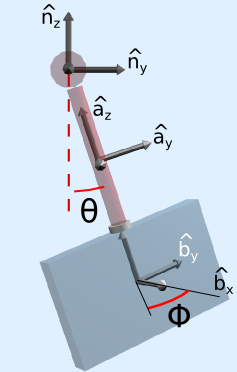
\includegraphics[width=0.95\columnwidth]{babyboot2.png}
\end{minipage}
%
\isolatedBuildFooter
